\section{HDSDP Software}\label{sec5}

\revised{{{\texttt{HDSDP}}} is written in \text{{\ttfamily{ANSI C}}}, coded according to the standard of commercial numerical software}, and provides a
self-contained user interface. While {{\texttt{DSDP5.8}}} serves as a sub-routine library, 
{{\texttt{HDSDP}}} is designed to be a stand-alone SDP solver and re-written to accommodate the 
new computational techniques and third-party packages. After the user inputs the data and invokes the optimization routine, {{\texttt{HDSDP}}} goes through several modules
including input check, pre-solving, two-phase optimization and post-solving. The modules are implemented independently and are sequentially organized in a pipeline. \revised{Compared with  {{\texttt{DSDP}}}, two most important computational improvements of {\hdsdp} lie in its conic KKT solver and its abstract linear system interface. To our knowledge, {\hdsdp} has the most advanced KKT solver among all the open-source SDP codes.
}

\subsection{Pre-solver}

One new feature of {{\texttt{HDSDP}}} is a special pre-solving module
 designed for SDPs. It inherits techniques from {{\texttt{DSDP5.8}}} and adds new strategies to work jointly with the optimization module. When the pre-solver is invoked, it first goes through the problem data $\{ \mathbf{A}_i \}$ for two rounds to detect the possible low-rank structure. The first round uses Gaussian elimination for rank-one structure and the
second round applies eigenvalue decomposition from \text{{\ttfamily{Lapack}}}. Two
exceptions are when the data matrix is too dense or sparse. Unlike in {{\texttt{DSDP5.8}}} where eigen-decomposition is mandatory, matrices that are too dense to be eigen-decomposed efficiently will be skipped in {{\texttt{HDSDP}}}; if a matrix has very few entries, then the solution from {{\texttt{DSDP5.8}}} is applied: {\textbf{1)}} a permutation gathers the non-zeros to a much smaller dense block. {\textbf{2)}} dense eigen routines from \text{{\ttfamily{Lapack}}} applies. {\textbf{3)}} the inverse permutation recovers the decomposition.

After detecting the hidden low-rank structures, the pre-solver moves on to collecting the sparsity and rank information of the matrices. The information will be kept for the KKT analysis to be described in \textbf{Section \ref{sec:kktsolver}}.

%After detecting the hidden low-rank structures, the pre-solver moves on to
%the analysis of the KKT matrix $\mathbf{M}$: {\textbf{1)}}. the sparsity and rank
%information of the matrices are collected. {\textbf{2)}}. a permutation of
%$\{ \mathbf{A}_i \}$ is generated in descending order of sparsity.
%{\textbf{3)}}. for each row of $\mathbf{M}$, the flops using each of {\textbf{M1}}
%to {\textbf{M5}} technique is computed and the cheapest technique is
%recorded. The recorded techniques reduces the flops to set up $\mathbf{M}$ and
%accelerates the convergence.

Finally, the pre-solver scales down the large objective coefficients by their Frobenius norm and goes on to identify the following structures. {\textbf{1)}}. Implied trace: constraints imply
$\ensuremath{\operatorname{tr}} ( \mathbf{X} ) = \theta$. {\textbf{2)}}. Implied dual bound:
constraints imply $\mathbf{l} \leq \mathbf{y} \leq \mathbf{u}$. {\textbf{3)}}. Empty
primal interior: constraints imply $\ensuremath{\operatorname{tr}} ( \mathbf{X} \mathbf{a} \mathbf{a}^{\top}
) \approx 0$. {\textbf{4)}}. Empty dual interior: constraints imply
$\mathcal{A}^{*} \mathbf{y} = \mathbf{C}$. {\textbf{5)}}. Feasibility problem: $\mathbf{C} = \textbf{0}$. {\textbf{6)}}. Dense problem: whether all the constraint matrices are dense.
{\textbf{7)}}. Multi-block problem: whether there are many SDP cones. For each of the cases the solver adjusts its internal strategies to enhance its numerical stability and convergence.

\subsection{Two-phase Optimization}

Underly the procedure control of {\hdsdp} is a two-phase method which integrates the technique
embedding (\text{{\ttfamily{Phase A}}}) and dual-scaling (\text{{\ttfamily{Phase B}}}). \
\text{{\ttfamily{Phase A}}} targets feasibility certificate, while \text{{\ttfamily{Phase B}}} aims to efficiently drive a dual-feasible solution to optimality.

\begin{figure}[h]
\centering
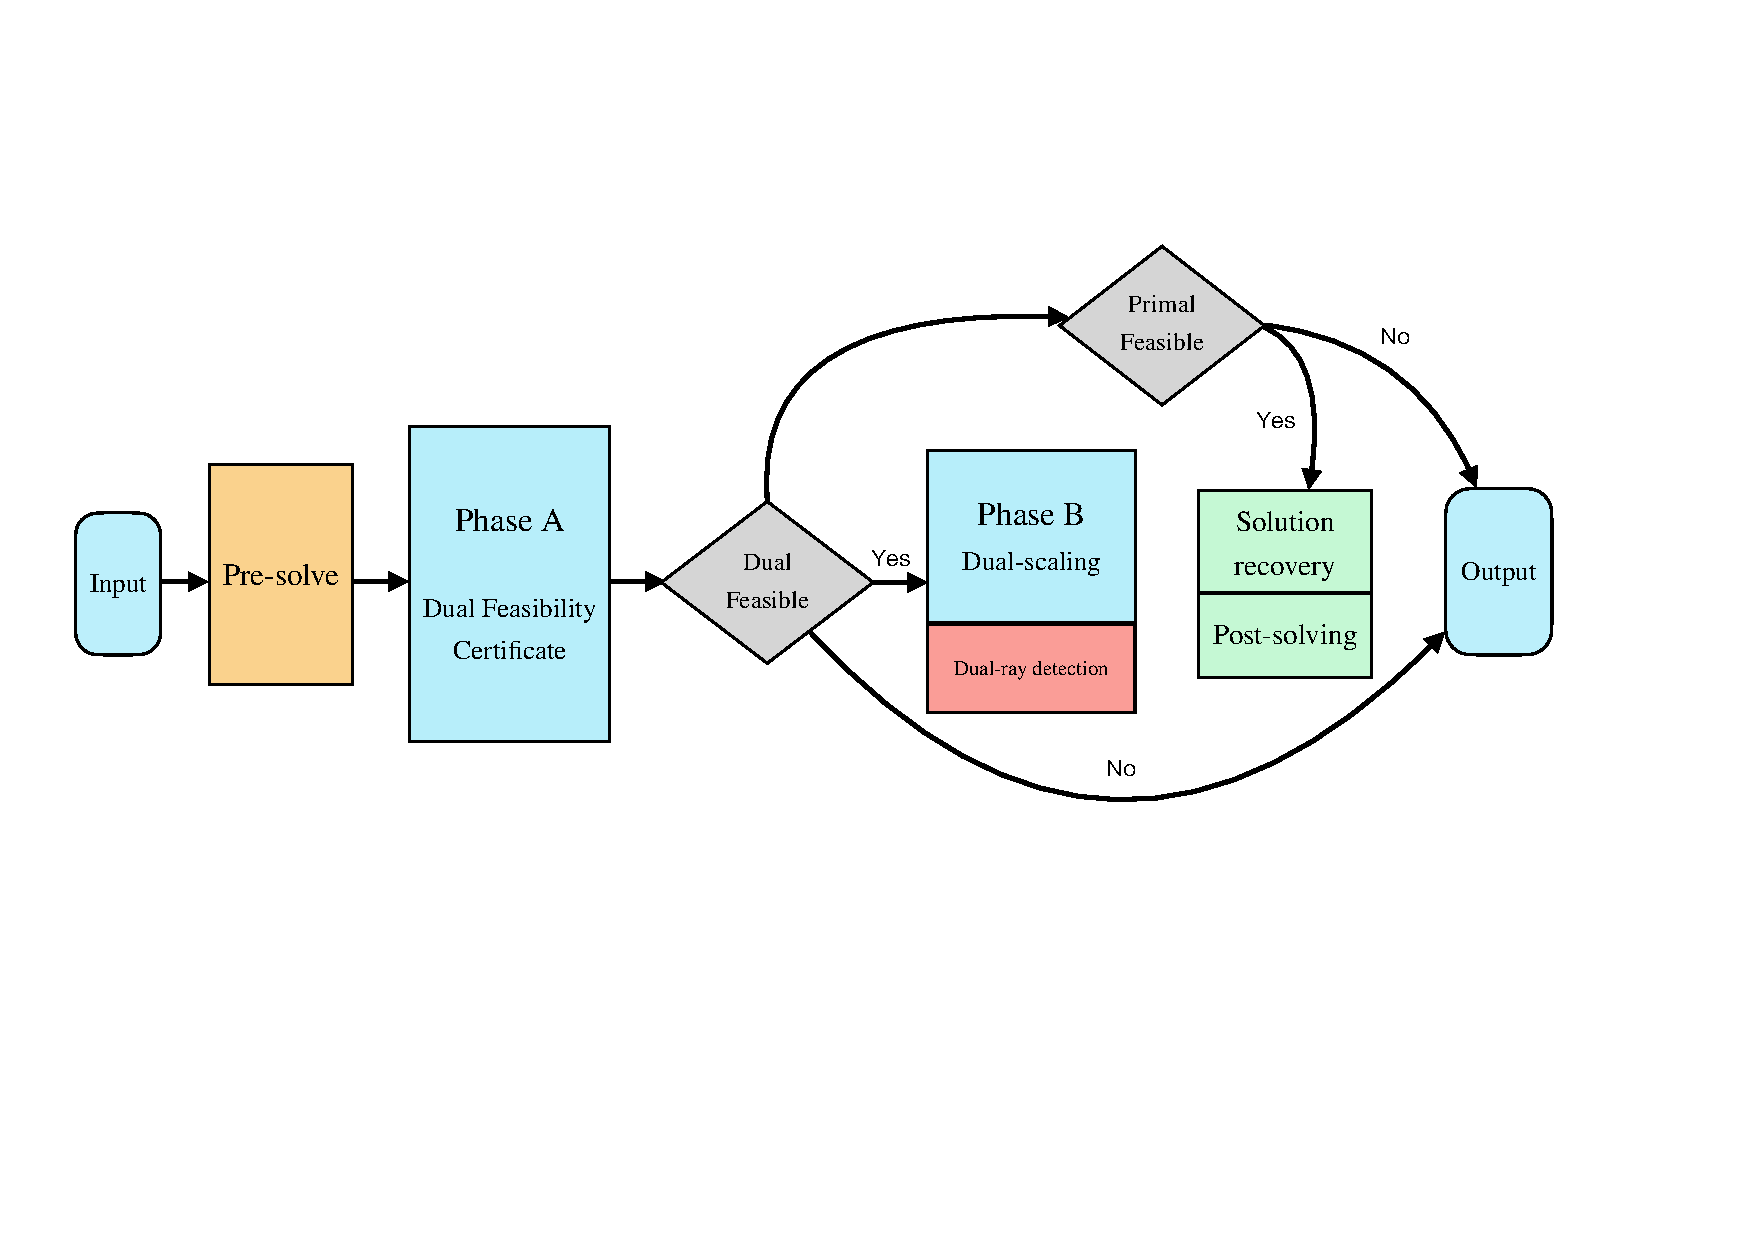
\includegraphics[scale=0.45]{fig.pdf}
  \caption{Pipeline of {{\texttt{HDSDP}}}}
\end{figure}

The two phases share the same backend computation routines but are
associated with different goals and strategies. {{\texttt{HDSDP}}} decides
which strategy to use based on the behavior of algorithm iterations.

\subsection{Conic KKT Solver} \label{sec:kktsolver}
\revised{
The most computationally intensive part in {{\texttt{HDSDP}}} is in the
the Schur complement matrix $\mathbf{M}$. In real-life applications, the SDP objective $\mathbf{C}$ often does not share the same sparsity or low-rank property as $\{ \mathbf{A}_i \}$. Therefore, the additional computation from $\mathcal{A} \mathbf{S}^{- 1} \mathbf{C} \mathbf{S}^{- 1}$ and $\langle \mathbf{C}, \mathbf{S}^{- 1} \mathbf{C} \mathbf{S}^{- 1} \rangle$ demands more efficient techniques to set up $\mathbf{M}$. }

\revised{Efficiency of setting up $\mathbf{M}$ depends mainly on two aspects: \textbf{1)}. the structure of the cones participating in forming the Schur complement, and \textbf{2)} the structure of the coefficients inside of each cone. To exploit both structures, KKT solver in {{\texttt{HDSDP}}} implements two abstract interfaces, one from conic coefficient to conic operations, the other from cone to $\mathbf{M}$. }

\revised{The first interface allows {{\texttt{HDSDP}}} to set up $\mathbf{M}$ faster, while the second allows the extension of dual-method to arbitrary cones. These two interfaces already appeared in {{\texttt{DSDP5.8}}}, but unifying them in a conic KKT solver makes the algorithm more compact. Till the date when this manuscript is written, four cones and five types SDP coefficients have been implemented by {{\texttt{HDSDP}}}. We refer the readers to the manual for a more detailed discussion of the conic interface.}

\revised{The interface from SDP coefficients to conic operations is directly relevant to the set up of $\mathbf{M}$. Using the rank and sparsity information from the pre-solver, {{\texttt{HDSDP}}} analyzes the Schur system and generates a permutation $\sigma (m)$ of the rows of $\mathbf{M}$.
The idea is to permute the most computationally-expensive matrices to the left-most position, and this is a direct extension of {\cite{fujisawa1997exploiting}}. }

\[ \left(\begin{array}{ccc}
     \langle \mathbf{A}_{\sigma (1)}, \mathbf{S}^{- 1} \mathbf{A}_{\sigma (1)} \mathbf{S}^{- 1}
     \rangle & \cdots & \langle \mathbf{A}_{\sigma (1)}, \mathbf{S}^{- 1}
     \mathbf{A}_{\sigma (m)} \mathbf{S}^{- 1} \rangle\\
     & \ddots & \vdots\\
     &  & \langle \mathbf{A}_{\sigma (m)}, \mathbf{S}^{- 1} \mathbf{A}_{\sigma (m)} \mathbf{S}^{- 1}
     \rangle
   \end{array}\right) \]\\
\revised{After deciding the permutation, for each row of the permuted system, {{\texttt{HDSDP}}} chooses one strategy out of a pool of five candidate techniques. We denote them by {\textbf{M1}} to {\textbf{M5}}, and they are efficient under different coefficient structures: Technique {\textbf{M1}} and {\textbf{M2}} are inherited from
{{\texttt{DSDP}}}. They exploit the low-rank structure of the coefficient data and
an eigen-decomposition of the data
$\mathbf{A}_i = \sum_{r = 1}^{\ensuremath{\operatorname{rank}} ( \mathbf{A}_i )} \lambda_{i r}
   \mathbf{a}_{i, r} \mathbf{a}^{\top}_{i, r}$
needs to be computed at the beginning of the algorithm; Technique {\textbf{M3}}, {\textbf{M4}} and {\textbf{M5}} exploit sparsity and need evaluation of $\mathbf{S}^{-1}$ {\cite{fujisawa1997exploiting}}.\\}

{\begin{minipage}{0.8\textwidth}
		{\textbf{KKT Technique M1}}
\begin{enumerate}[leftmargin=25pt]
  \item {\textbf{Setup}} $\mathbf{B}_{\sigma (i)} = \sum_{r =
  1}^{\ensuremath{\operatorname{rank}} ( \mathbf{A}_{\sigma (i)} )} \lambda_r \big( \mathbf{S}^{- 1}
  \mathbf{a}_{\sigma (i), r} \big) ( \mathbf{S}^{- 1} \mathbf{a}_{\sigma (i), r})^{\top}$.
  
  \item {\textbf{Compute}} $M_{\sigma (i) \sigma (j)} = \langle
  \mathbf{B}_{\sigma (i)}, \mathbf{A}_{\sigma (j)} \rangle, \text{for all } j \geq i$.
\end{enumerate}
{\textbf{KKT Technique M2}}
\begin{enumerate}[leftmargin=25pt]
  \item {\textbf{Setup}} $\mathbf{S}^{- 1} \mathbf{a}_{\sigma (i), r}, r = 1, \ldots,
  r_{\sigma (i)}$.
  \item {\textbf{Compute}} $M_{\sigma (i) \sigma (j)} =  \sum_{r =
  1}^{\ensuremath{\operatorname{rank}} ( \mathbf{A}_{\sigma (i)} )} \lambda_r ( \mathbf{S}^{- 1}
  \mathbf{a}_{\sigma (i), r} )^{\top} \mathbf{A}_{\sigma (j)} ( \mathbf{S}^{- 1}
  \mathbf{a}_{\sigma (i), r} )$.
\end{enumerate}
{\textbf{KKT Technique M3}}
\begin{enumerate}[leftmargin=25pt]
  \item {\textbf{Setup}} $\mathbf{B}_{\sigma (i)} = \mathbf{S}^{- 1} \mathbf{A}_{\sigma
  (i)} \mathbf{S}^{- 1}$
  \item {\textbf{Compute}} $M_{\sigma (i) \sigma (j)} = \langle
  \mathbf{B}_{\sigma (i)}, \mathbf{A}_{\sigma (j)} \rangle, \text{for all } j \geq i$
\end{enumerate}

{\textbf{KKT Technique M4}}
\begin{enumerate}[leftmargin=25pt]
  \item {\textbf{Setup}} $\mathbf{B}_{\sigma (i)} = \mathbf{S}^{- 1} \mathbf{A}_{\sigma
  (i)}$
  
  \item {\textbf{Compute}} $M_{\sigma (i) \sigma (j)} = \langle
  \mathbf{B}_{\sigma (i)} \mathbf{S}^{- 1}, \mathbf{A}_{\sigma (j)} \rangle, \text{for all } j
  \geq i$
\end{enumerate}
{\textbf{KKT Technique M5}}
\begin{enumerate}[leftmargin=25pt]
  \item {\textbf{Compute}} $M_{\sigma (i) \sigma (j)} = \langle \mathbf{S}^{-
  1} \mathbf{A}_{\sigma (i)} \mathbf{S}^{- 1}, \mathbf{A}_{\sigma (j)} \rangle, \text{for all } j \geq
  i$ directly.
\end{enumerate}
\end{minipage}}

\begin{table}[h]
  \centering
  \caption{Approximate flops for each strategy. $f_i$ is the number of nonzeros of $\mathbf{A}_i$; $r_i$ is rank of $\mathbf{A}_i$, $\kappa$ is the slow down ratio of discontinuous memory access}
  \begin{tabular}{ccc}
  \toprule
    KKT Technique & Flops & Extra cost \\
    \midrule
    {\textbf{M1}} & $r_{\sigma (i)} (n^2 + 2 n^2) + \kappa \sum_{j \geq i}
    f_{\sigma (j)}$ & 0\\
    {\textbf{M2}} & $r_{\sigma (i)} ( n^2 + \kappa \sum_{j \geq i}
    f_{\sigma (j)} )$ & 0 \\
    {\textbf{M3}} & $n \kappa f_{\sigma (i)} + n^3 + \sum_{j \geq i} \kappa
    f_{\sigma (j)}$ & $n^3$ \\
    {\textbf{M4}} & $n \kappa f_{\sigma (i)} + \sum_{j \geq i} \kappa (n +
    1) f_{\sigma (j)}$ & $n^3$\\
    {\textbf{M5}} & $\kappa (2 \kappa f_{\sigma (i)} + 1)  \sum_{j \geq i}
    f_{\sigma (j)}$ & $n^3$\\
    \bottomrule
  \end{tabular}
\end{table}

\revised{This newly developed KKT solver improves the speed of {{\texttt{HDSDP}}} on a broad set of instances. And to our knowledge {{\texttt{HDSDP}}} is the first SDP software that simultaneously incorporates all the commonly-used Schur complement strategies.}

\subsection{Linear System Interface and Parallel Computation}

\revised{
Linear system solving is the core of any interior point software, and most of the linear system solvers nowadays provide support for multi-threading. In {{\texttt{HDSDP}}}, matrix decomposition is 
required for both the dual matrix $\mathbf{S}$ and the Schur complement $\mathbf{M}$, both of which would need different decomposition routines based on matrix data structure and numerical conditioning. To meet this requirement, {{\texttt{HDSDP}}} adopts a plug-in type abstract linear system interface which allows users to adopt any linear system routine. \textbf{Table \ref{table:linsys}} summarizes the routines supported by {{\texttt{HDSDP}}} and by default the multi-threaded Intel MKL routines are adopted and threading is controlled by a user-specified parameter.
\begin{table}[h]
  \caption{Linear systems in {{\texttt{HDSDP}}}} \label{table:linsys}
  \begin{tabular}{cccc}
      \toprule
    Linear system type & Implementation & Parallel & Available in Public \\
      \midrule
    Dense Restarted PCG & {{\texttt{HDSDP}}} & Yes & Yes \\
    Positive definite sparse direct & (MKL) Pardiso \cite{wang2014intel} & Yes & No\\
    Quasi-definite sparse direct & \texttt{COPT} \cite{copt} & Yes & No\\
    Positive-definite dense direct & \texttt{COPT} \cite{copt} & Yes & No\\
    Positive definite sparse direct & SuiteSparse \cite{davis2006direct} & No & Yes\\    
    Positive definite dense direct  & (MKL) Lapack \cite{wang2014intel} & Yes & Yes\\
    Symmetric indefinite dense direct & (MKL) Lapack \cite{wang2014intel} & Yes & Yes\\
    \bottomrule
  \end{tabular}
\end{table}}

\revised{Aside from the third-party routines, {{\texttt{HDSDP}}} itself implements a pre-conditioned conjugate gradient (CG) method with restart to solve the Schur complement system. The maximum number of iterations is
chosen around $50 / m$ and is heuristically adjusted. Either the diagonal of
$\mathbf{M}$ or its Cholesky decomposition is chosen as pre-conditioner and
after a Cholesky pre-conditioner is computed, {{\texttt{HDSDP}}} reuses it for 
the consecutive solves till a heuristic determines that the current
pre-conditioner is outdated. When the algorithm approaches optimality, $\mathbf{M}$
might become ill-conditioned and {{\texttt{HDSDP}}} switches to {\textsf{LDL}} decomposition in case Cholesky fails.}

%\subsection{Iteration Monitor}
%
%To help the users capture the progress of the solver, {{\texttt{HDSDP}}}
%prints related information to the screen at different stages of optimization. 
%\begin{lstlisting}
%--------------------------------------------------------------------------------------
%| Start presolving 
%| - XXX completes in 0.001 seconds 
%| - Matrix statistics ready in 0.000 seconds 
%|    Schur Re-ordering: M1: 0  M2: 3000  M3: 0  M4: 1  M5: 0 
%| - Special structures found 
%|    tr(X) = 3.00e+03 : Bound of X fixed 
%| Presolve Ends. Elapsed Time: 0.371 seconds 
%--------------------------------------------------------------------------------------
%\end{lstlisting}
%While pre-solving, {{\texttt{HDSDP}}} prints time statistics when certain operation
%is done. Specially, the row
%\begin{tmcode}
%      Schur Re-ordering: M1: 0  M2: 3000  M3: 0  M4: 1  M5: 0
%\end{tmcode}
%indicates how many times each Schur complement technique is applied and if
%special SDP structures are detected, they are also printed to the screen.
%\begin{tmcode}
%      tr(X) = 3.00e+03 : Bound of X fixed.
%\end{tmcode}
%When the pre-solving ends, {{\texttt{HDSDP}}} prints matrix statistics
%including type and sum of norm. Also, the solver internally adjusts its parameters
%based on the collected information and display them to the user. 
%
%\begin{lstlisting}
%--------------------------------------------------------------------------------------
%| Matrix statistics [Including C]: 
%--------------------------------------------------------------------------------------
%|     Zero |   Sparse |    Dense |   Rank-1 |      |A|    |      |b|    |      |C|     
%--------------------------------------------|-----------------------------------------
%|        0 |        1 |        0 |     3000 |  3.0000e+03 |  3.0000e+03 |  1.2000e+04 
%--------------------------------------------------------------------------------------
%| Parameter Summary: 
%--------------------------------------------------------------------------------------
%| Rhon [1.0, 10.0]: 5 
%| Golden linesearch \{0, 1\}: 0 
%| Primal relaxation penalty (0.0, inf): 1e+07 
%| Time limit (0.0, inf): 15000 
%| Corrector A: 4  Corrector B: 0 
%--------------------------------------------------------------------------------------
%| DSDP is initialized with Ry = -1.225e+05 * I                                                     
%| DSDP Phase A starts. Eliminating dual infeasibility                                              
%--------------------------------------------------------------------------------------
%\end{lstlisting}
%
%After pre-solving, {{\texttt{HDSDP}}} enters optimization, invokes HSD embedding (\text{{\ttfamily{Phase A}}}), and prints logs.
%
%\begin{lstlisting}
%--------------------------------------------------------------------------------------
%| Iter |     pObj |     dObj |     dInf |     k/t |      mu |   step |   Pnorm |   E |
%--------------------------------------------------------------------------------------
%|    1 |  1.0e+05 |  0.0e+00 | 6.71e+06 | 1.0e+00 | 4.0e+04 |   0.00 | 1.0e+20 |     |
%|    2 |  2.4e+08 | -7.3e+08 | 0.00e+00 | 1.0e+00 | 3.8e+04 |   1.00 | 1.1e+02 |   * |
%--------------------------------------------------------------------------------------	
%\end{lstlisting}
%
%
%\begin{table}[h]
%\centering
%  \begin{tabular}{r|l}
%        
%    \text{{\ttfamily{Iter}}} & the iteration number\\
%    \text{{\ttfamily{pObj}}} & the primal objective bound\\
%    \text{{\ttfamily{dObj}}} & the dual objective \\
%    \text{{\ttfamily{k/t}}} & $\kappa / \tau$ from the embedding\\
%    \text{{\ttfamily{mu}}} & the current barrier parameter\\
%    \text{{\ttfamily{step}}} & stepsize $\alpha$ taken\\
%    \text{{\ttfamily{Pnorm}}} & the proximity to the central path\\
%    \text{{\ttfamily{E}}} & event monitor\\
%        
%  \end{tabular}
%  \caption{Iteration monitor of Phase \text{{\ttfamily{A}}}}
%\end{table}
%
%When \text{{\ttfamily{Phase A}}} finds a dual-feasible solution, {{\texttt{HDSDP}}}
%collection the solution statistics to adjust the parameters for
%dual-scaling in \text{{\ttfamily{Phase B}}}, prints related information and performs re-start.
%
%\begin{lstlisting}
%--------------------------------------------------------------------------------------
%| DSDP Phase A ends with status: DSDP_PRIMAL_DUAL_FEASIBLE                                         
%| Elapsed Time: 0.535 seconds                                                                   
%--------------------------------------------------------------------------------------
%| DSDP Phase A certificates primal-dual feasibility                                                
%| Primal relaxation penalty is set to  2.449e+06 
%| Perturbing dual iterations by  0.000e+00 
%| DSDP Phase B starts. Restarting dual-scaling                                                     
%| Heuristic start: mu:  2.177e+04 pObj:  2.450e+08  dObj: -7.346e+08                              
%--------------------------------------------------------------------------------------
%\end{lstlisting}	
%
%The log from \text{{\ttfamily{Phase B}}} is similar to \text{{\ttfamily{Phase A}}} but
%\text{{\ttfamily{dInf}}} is now replaced by \text{{\ttfamily{pInf}}} to characterize primal
%infeasibility. Also, \text{{\ttfamily{k/t}}} is dropped from log since the embedding
%is not applied.
%
%\begin{lstlisting}
%--------------------------------------------------------------------------------------
%| Iter |        pObj |        dObj |       pInf |       mu |   step |    Pnorm |   E |
%--------------------------------------------------------------------------------------
%|    1 |  2.4500e+08 | -7.3462e+08 |  3.001e+03 | 2.18e+04 |   1.00 |  1.1e+02 |     |
%|    2 |  2.4500e+08 | -3.6742e+07 |  3.001e+03 | 2.18e+04 |   0.09 |  5.6e+02 |     |
%|    3 |  1.3061e+08 | -1.8487e+06 |  8.915e-03 | 3.72e+03 |   0.41 |  1.3e+02 |   P |
%...
%|   14 | -1.1997e+04 | -1.2000e+04 |  9.510e-11 | 4.66e-06 |   0.00 |  9.4e+00 |   P |
%|   15 | -1.1999e+04 | -1.2000e+04 |  1.902e-12 | 9.32e-07 |   0.02 |  5.1e+01 |   F |
%--------------------------------------------------------------------------------------
%\end{lstlisting}
%
%When \text{{\ttfamily{Phase B}}} converges, the solver extracts the solution status,
%recovers primal feasible solution (if available) and briefly prints solution
%and time statistics.
%
%\begin{lstlisting}
%--------------------------------------------------------------------------------------
%| DSDP Phase B ends with status: DSDP_INTERNAL_ERROR                                               
%| Elapsed Time: 5.960 seconds                                                                   
%--------------------------------------------------------------------------------------
%| DSDP Ends.                                                                                        
%--------------------------------------------------------------------------------------
%| Primal solution is extracted.                                                                    
%| Final pObj: -1.19993e+04   dObj: -1.20000e+04 
%--------------------------------------------------------------------------------------
%| DSDP Time Summary: 
%--------------------------------------------------------------------------------------
%|           Event |    Time(s) | 
%--------------------------------------------------------------------------------------
%|        Presolve |      0.371 | 
%|  Phase A (iter) |      0.535 | (2) 
%|  Phase B (iter) |      5.960 | (15) 
%|           Get X |      0.809 | 
%|       Postsolve |      0.000 | 
%|             All |      7.675 | (17) 
%--------------------------------------------------------------------------------------
%\end{lstlisting}
%
%Compared to other IPM solvers, {{\texttt{HDSDP}}} tends to display more information so that the users better 
%understand structures and features of the SDP instance. We believe that knowledge of
%the problem structure would assist the users when customzing the solver for their applications.
